% When we observe an animal grappling with the decision to either explore or exploit, we often imagine this decision is based on reward. For example, if a bee goes in a familiar direction \textit{to gather nectar}, it is said to be exploiting past knowledge for environmental reward. If it goes in an unfamiliar direction \textit{to gather nectar}, it is said to be exploring for reward. Because the environment is partly unkown to the bee, it cannot rationally choose which action it should be doing, exploiting or exploring \textit{to gain more reward}. It is this uncertainty \textit{about returning the most rewards} that makes explore-exploit choices a dilemma. It is also this uncertainty which ensures there is no tractable mathematical solution for explore-exploit questions about reward \citep{Thrun1992a,Dayan1996,Ishii2002,Simsek2006,Gershman2018b}. We illustrate this view in Fig. \ref{fig:bee}a.

% The choice between exploring and exploiting is indeed faced routinely by learners of all kinds, including foraging bees, business organizations, humans, worms, monkeys, rodents, birds, children, and computer algorithms \citep{Gupta2006,Sutton2018,Woodgate2017,Lee2011a,Schulz2018a,Calhoun2014,Wang2019,Sumner2019,Auersperg2015}. But is reward really fundamental to it? Because in the natural world exploration already finds two explanations. If there is no reason to expect a reward, exploration is described theoretically as a search for information, what we will call curiosity \citep{Berlyne1950,Schmidhuber1991,Kidd2015,deAbril2018,Jaegle2019,Friston2016}. On the other hand, if reward is expected, then exploration gets re-interpreted as we described above, as a search for reward, and this specific interpretation is what leads the famous dilemma \citep{Kelly1956,Berger-Tal2014,Dayan1996,Thrun1992,Mehlhorn2015,Kobayashi2019}. 

% Why curiosity? Curiosity is a rational behavoir \cite{Rich2016a}, or so we argue. Curiousity is just as important for survival as reward collection \cite{Thrun1992}. Curiosity is a primary drive in most, if not all, animals \cite{Inglis2001}. It is as strong, if not sometimes stronger, than the drive for reward \cite{Loewenstein1994,Kidd2015,Gottlieb2018}. Curiosity, as an algorithm, is highly effective at solving optimization problems \cite{Schmidhuber1991,Pathak2017,Stanton2018,Lehman201,Mouret2011b1,Fister2019,Mouret2015,Colas2020,Cully2015,Pathak2017,Schwartenbeck2019.Laversanne-Finot2018}. In short, curiosity is necesssary, omnipresent, and effective.

%  TODO - Need oprn-field/maze cites with no reward
Exploration during behavior can have two very different explanations depending on whether an animal or artificial agent might receive a reward. If there is no reason to expect a reward, exploration is treated as a search for information, or curiosity \cite{Berlyne1950,Schmidhuber1991,Kidd2015,Jaegle2019,Friston2016,Sumner2019,Calhoun2014,Wang2019,Auersperg2015}. For example, when a rat is placed in a new environment it will explore even if no food and water is present, or expected \cite{TODO}. If however reward is expected rhis exploration is interpreted as a search to maximize reward \cite{Gupta2006,Sutton2018,Woodgate2017,Lee2011a,Schulz2018a}. % TODO - more cites...

An open problem in the decision sciences it to unify both kinds of exploration with exploitation, the policy of choosing the most rewarding action. This is difficult because exploration for reward is inhrently uncertain. When it is combined with exploitation, the conflict between them creates an irrational conflict, that leads to a dilemma \citep{Kelly1956,Berger-Tal2014,Dayan1996,Thrun1992,Mehlhorn2015,Kobayashi2019} (as illustrated in Fig. \ref{fig:bee}a).

Our goal in this paper is to maximize the return of reward. But have come to believe curiosity is better general goal for exploration, rather than searching to optimize reward direclty. This ``curiosity trick'' is a counterintuitive suggestion. Why would it be better to search only to learn, instead of optimizing for reward? In this paper we will prove that exploration is often better handled by a curiosity search--even when the goal is to collect the most reward. We illustrate this view, and our trick, in Fig. \ref{fig:bee}b. We justify the use of curiosity because it is a primary drive in most, if not all, animals \cite{Loewenstein1994,Inglis2001}. It is as strong, if not sometimes stronger, than the drive for reward \cite{Loewenstein1994,Kidd2015,Gottlieb2018}.

\begin{figure}
	\begin{fullwidth}
	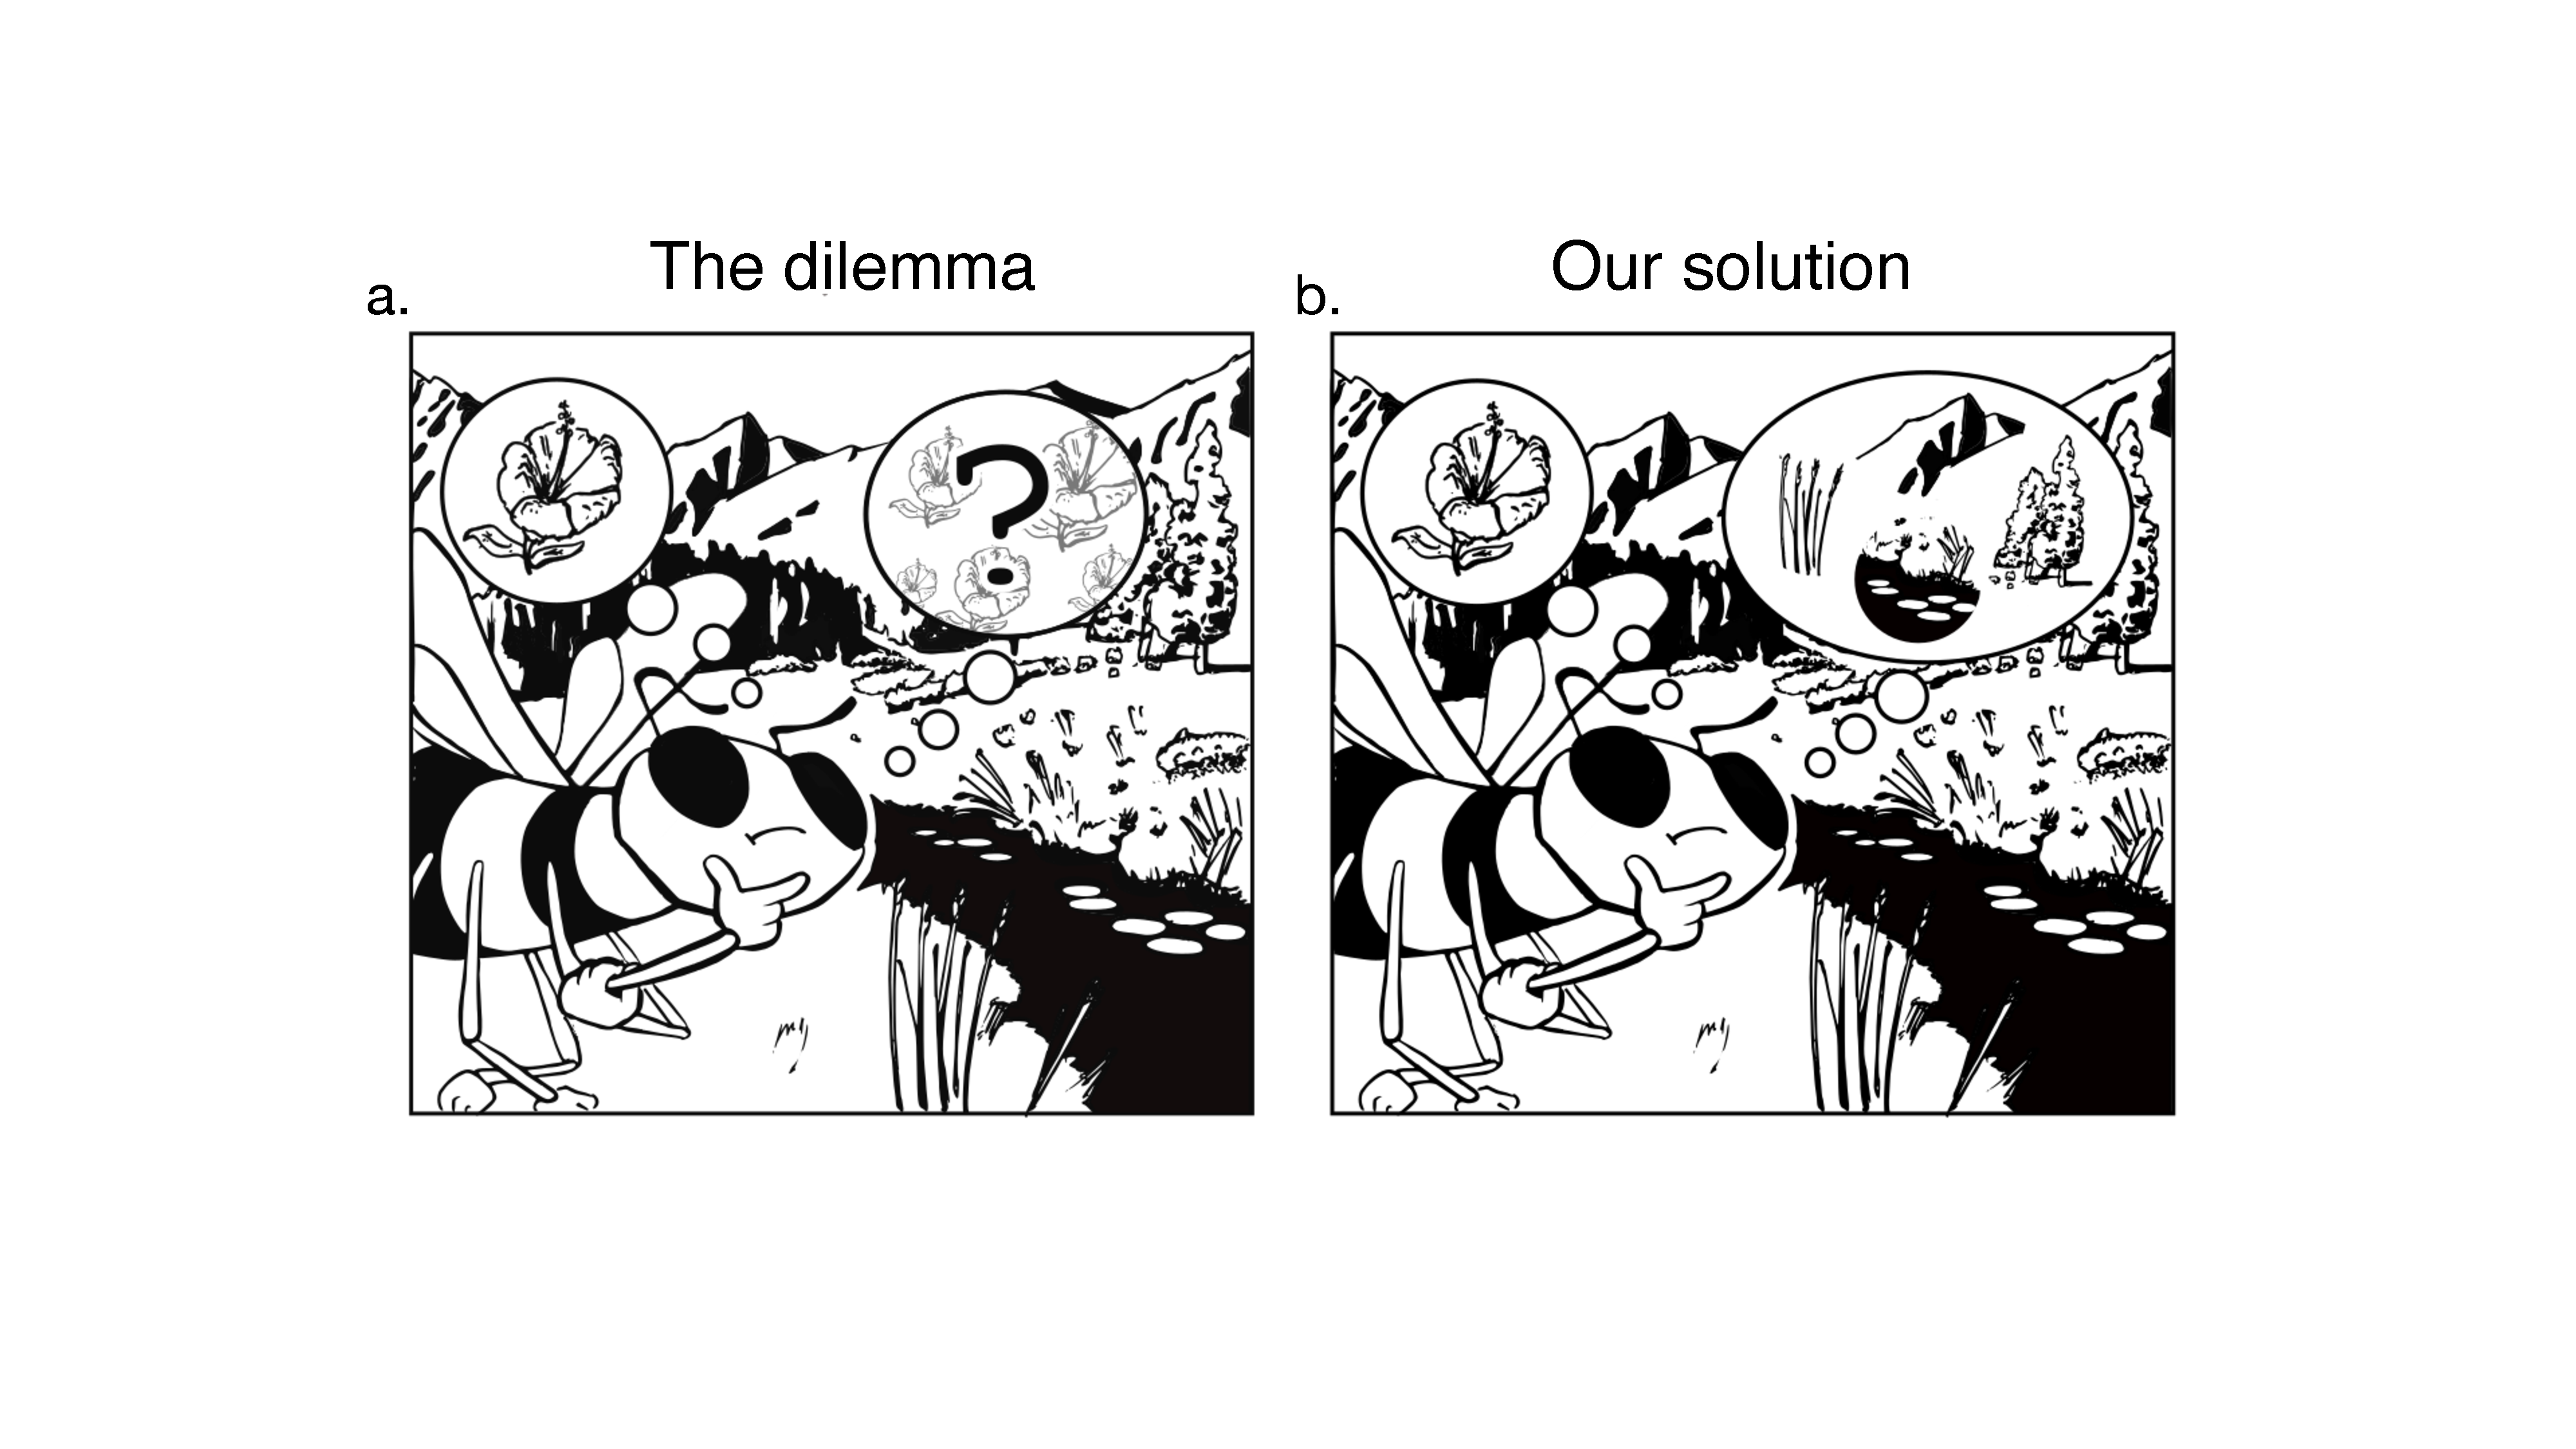
\includegraphics[width=.55\linewidth]{dilemma-draft-elife/img/bee.pdf} 
	\caption{Two views of exploration and exploitation. \textbf{a}. The classic dilemma: either exploit an action with a known reward (e.g., return to the previous flower) or explore other actions on the chance they will return a better outcome. The central challenge here is that the outcome of exploration is uncertain, and filled with questions. \textbf{b}. An alternative view of the dilemma, with two goals: either maximize rewards \textit{or} maximize information value with a curious search of the environment. \textit{Artist credit}: Richard Grant.}
	\label{fig:bee} 
	\end{fullwidth}
\end{figure}

The first half of this paper is devoted to developing a new mathmtical view of curiosity, and a new understanding of ideal curious search. This effort will let us make a new contribution to information theory--defining subjective information value without considering meaning. The second half uses these first results to prove pure curiosity can generate an optimal value solution for all explore-exploit decisions. We prove this with both theory, and simulation experiments.
